\chapter{Student evaluation}\label{ap:student}

Teaching should not be considered independently from learning; when evaluating the effectiveness of a teaching practice it is necessary to listen to feedback from students and peers \citep[chapter 7]{Ramsden1992}. In this appendix, I discuss feedback from my students. In \apref{peer} I include feedback on my teaching from peers. Students are well-placed to evaluate their own learning, and frequently values the same things as teachers \citep[chapter 6]{Ramsden1992}.

In \secref{2014-15students} I describe my students and in \secref{questions} I explain how I collected feedback from them. This feedback is analysed in \secref{results}, and I summarise my conclusions in \secref{student-conc}.

\section{2014/2015 students}\label{sec:2014-15students}

This academic year I taught a total of nine students; I had one tutorial group of four and another of five. The fifth member of the second group joined at the start of the Spring term. Since their experience is anomalous and they did not complete the practice essay, their feedback is not included in the analysis presented here. Amongst the remaining eight students, two are female (one in each group), one is an international student (with English as a second language), and none have disclosed special learning needs. The students represent a range of abilities as assessed from their first-year marks, covering the span from 2.ii to high 1st.

\section{Collecting feedback}\label{sec:questions}

\subsection{Overview}

I asked for feedback from my students at the start of the Spring term to coincide with the PRTs (see \apref{plan}). I tried to link the ideas of reviewing my progress with reviewing theirs to make the topic more approachable. I asked them to complete an anonymous, electronic questionnaire. This is explained in \secref{form1}. Most did this ahead of the PRT, so I was able to ask them some additional follow-up questions, as well as asking them if there was anything further they would like to discuss.\footnote{\citet[chapter 11]{Ramsden1992}, emphasised that one must not use questionnaires blindly to assess quality of teaching.}

I asked the students to complete a further, shorter questionnaire at the end of the Spring term, once they had received feedback from their essays. This is explained in \secref{form2}. I have not had opportunity to follow this up; however, I will ask for any further comments at the end of the year.

\subsection{First Questionnaire}\label{sec:form1}

This questionnaire was divided into four sections: A.\ tutorials, B.\ communication skills, C.\ essay preparation, and D.\ general comments. The first three go from a broad overview of how students view tutorials, to how I teach essay writing within tutorials. The final section gives students opportunity to give some more general feedback on tutorials and address any other issues. The questions are described in \tabref{form1}, in detail:
\begin{itemize}
\item Question 1 tries to gauge student interest in tutorials. If they are highly valued, students should be motivated to work for them, whereas if they are not, they would be unwilling to put in extra time to prepare for them (and hence be reluctant to commit time to the practice essay).
\item Question 2 asks how happy students are in tutorials. I do not expect them to be entirely relaxed, since there is always some pressure associated with answering questions. However, I try to maintain an informal atmosphere so that students are comfortable contributing to discussions and, in particular, asking questions on areas of weakness.\footnote{Use of humour can improve retention and ease anxiety \citep[e.g.,][and references therein]{Korobkin1988,Lesser2008}, and I incorpe jokes and anecdotes (about my own studies and famous physicists) into tutorials.} I hope to establish a good teacher--student relationship, which can have positive learning outcomes \citep{Cornelius-White2007}.
\item Questions 3 and 4 assess my competency as a physicist and a teacher respectively \citep[cf.][figure 4.15, section A]{Brown1988}. I am confident in my subject knowledge, but included question 3 to try to separate subject-specific knowledge from the ability to teach it. Question 4 is similar to question 18 of \citet[appendix]{Ramsden1992}.
\item Questions 5 and 6 attempt to gauge the effectiveness of tutorials and how much benefit students are receiving from them \citep[cf.][figure 4.15, section B]{Brown1988}.
\item Question 7 allows for further comments on tutorials.
\item Questions 8 and 9 ask how valued communication skills are. I have specified a division between physics and life in general to assess whether students see communications skills as integral to their mastery of physics; as a hard science, students may value mathematical or analytical skills over softer skills \citep[cf.][figure 5.4]{Kolb1984}. If students value communication skills, they should be more motivated to spend time working on them.
\item Questions 10 and 11 check if students are happy with the time spent on communication skills. Time in tutorials is limited, hence it is important that students are happy with how this is spent \citep[cf.][appendix, question 30]{Ramsden1992}; if students think too much time is spent on communications skills, they would be unwilling to spend time on a formative essay.
\item Questions 12 and 13 ask students to reflect on their skills \citep[cf.][figure 4.15, section C]{Brown1988}, and hopefully determine how beneficial the activities have been this year.
\item Question 14 allows them to add further comments on communication skills.
\item Questions 15 and 16 assess the usefulness of the formative essay. The former question takes a holistic look at the exercise, and could include the benefit of practising writing; the latter looks just at the quality of the feedback.
\item Question 17 and 18 look at the usefulness of the blog post. A like to \url{http://cplberry.com/right-good/} was provided with the questions, and I hoped that these question would encourage students to read (or reread) the post, and hopefully take something from it.
\item Question 19 asks about confidence in referencing. I expected this topic to be troublesome (see \apref{threshold}).
\item Question 20 links the essay and presentation. I hoped to link these aspects of communication together (\secref{timetable}), and this question should help to quantify how successful this was and potentially encourage students to reflect upon this connection further.
\item Question 21 closes the section on essay writing, asking for any further comments.
\item Questions 22, 23 and 24 ask for suggestions for things to be included, continued or stopped in tutorials.
\item Question 25 asks for any other feedback.
\end{itemize}
\begin{table}\scriptsize
\centering
\begin{tabular}{c c p{2in} p{2in}}
\toprule
\multicolumn{1}{c}{Question} & \multicolumn{1}{c}{Section} & \multicolumn{1}{c}{Question} & \multicolumn{1}{c}{Response} \\
\midrule 
\hphantom{0}1 & \multirow{12}{*}{A} & How important are tutorials? & Not at all $0 \leftrightarrow 5$ Extremely \\
\hphantom{0}2 &		& How comfortable are you in tutorials? & Uncomfortable, self-conscious, unhappy $0 \leftrightarrow 5$ Happy, respected, relaxed \\
\hphantom{0}3 & 	& How knowledgeable is the tutor? & Does not know the subject $0 \leftrightarrow 5$ Confident in subject area \\
\hphantom{0}4 &		& How are the tutor's explanations? & Incomprehensible, useless $0 \leftrightarrow 5$ Clear, understandable \\
\hphantom{0}5 & 	& How well do tutorials fit your needs? & Not at all $0 \leftrightarrow 5$ Perfectly \\
\hphantom{0}6 & 	& How much have you learnt from tutorials? & Nothing $0 \leftrightarrow 5$ A lot \\
\hphantom{0}7 &		& Any comments on your answers to these questions? & Free text \\
\midrule
\hphantom{0}8 & \multirow{16}{*}{B} & As a physicist, how valued are communication skills? & Not at all $0 \leftrightarrow 5$ Extremely highly \\
\hphantom{0}9 &	& How important are communication skills in life in general? & Not at all $0 \leftrightarrow 5$ Vital \\
10 &	& Outside of tutorials, does the course syllabus include the right amount time teaching communication skills? & Not enough $0 \leftrightarrow 5$ Too much \\
11 & 	& In tutorials, does the syllabus include the right amount of time teaching communication skills? & Not enough $0 \leftrightarrow 5$ Too much \\
12 & 	& How confident were you in your communication skills at the start of the year? & Not at all $0 \leftrightarrow 5$ Extremely \\
13 &	& How much have your skills improved since the start of the year? & Not at all $0 \leftrightarrow 5$ Lots \\
14 &	& Any comments on your answers to these questions? & Free text \\
\midrule
15 & \multirow{15}{*}{C} & Was writing a practice essay a useful experience? & Not at all $0 \leftrightarrow 5$ Absolutely \\
16 &	& How good was the feedback from your practice essay? & Unhelpful, unclear, unconstructive $0 \leftrightarrow 5$ Useful, detailed, understandable \\
17 &	& Have you read the blog post on essay writing? & No $0 \leftrightarrow 5$ In great detail \\
18 &	& How useful is a written resource like the blog post? & Not at all $0 \leftrightarrow 5$ Extremely \\
19 &	& How confident were you with referencing at the start of the year? & Not at all $0 \leftrightarrow 5$ Completely \\
20 &	& How much have you learnt from giving a presentation that can be applied to essay writing? & Nothing $0 \leftrightarrow 5$ Lots \\
21 &	& Any comments on your answers to these questions? & Free text \\
\midrule
22 & \multirow{8}{*}{D} & Is there something new you would like to start doing in tutorials? & Free text \\
23 &	& Is there something you would like to definitely continue doing in tutorials? & Free text \\
24 &	& Is there something you would like to stop doing in tutorials? & Free text \\
25 &	& Is there any other feedback you would like to give? & Free text \\
 \bottomrule
\end{tabular}
\caption{Details of the first student feedback questionnaire. Responses were collected anonymously online. Questions are split into four sections: A.\ tutorials, B.\ communication skills, C.\ essay preparation, and D.\ general comments. Questions were either answered by selected a number $0 \leftrightarrow 5$ ($0$, $1$, $2$, $3$, $4$ or $5$), or with free-form text. Results are discussed in \secref{results}.}\label{tab:form1}
\end{table}

\subsection{Second Questionnaire}\label{sec:form2}

The second questionnaire was briefer, it was divided into two sections: E.\ essays and F.\ course components. The first asks students to reflect on their essay writing having completed the assignment and received feedback. The second is a follow-up to question 1 from the first questionnaire. The questions are described in \tabref{form2}, in detail:
\begin{itemize}
\item Question 26 asks for students to comment on their essay mark. This is intended to assess whether students have achieved well without asking for their mark, which could identify them.
\item Questions 27 and 28 aim to evaluate how students used feedback from the formative assessment. This would help to quantify how useful completing the practice essay was.
\item Questions 29 and 30 do the same as 2 and 3, but for the blog posts.
\item Question 31 asks if feedback would be used in the future. It is possible students who had not made use of feedback up to this point, might not have realised its value. This question also attempts to make the connection that feedback from the essays could be useful for other tasks, such as project reports or dissertations.
\item Question 32 provides opportunity to provide further feedback on essay writing.
\item Question 33 asks students to reflect upon how they learn and to evaluate the effectiveness of different aspects of their course. The options are randomly on the questionnaire. Like question 1 from the first questionnaire, this intends to determine how much students value tutorials, but now it is relative to other aspects of the course. Additionally, encouraging students To consider how they learn best may help them establish an effective educational strategy, which is especially important ahead of planning their revision time and going on to third year where they receive less pastoral support.
\item Question 34 closes with the opportunity for further comments.
\end{itemize}
\begin{table}\scriptsize
\centering
\begin{tabular}{c c p{2in} p{2in}}
\toprule
\multicolumn{1}{c}{Question} & \multicolumn{1}{c}{Section} & \multicolumn{1}{c}{Question} & \multicolumn{1}{c}{Response} \\
\midrule 
26 & \multirow{17}{*}{E} & How happy are you with your essay mark & Extremely disappointed $0 \leftrightarrow 5$ Extremely pleased \\
27 &		& Did you use feedback from the practice essay when writing the assessed essay? & Yes or no \\
28 & 	& If you did use the feedback, was it useful? If you didn't, might it have been useful? & Completely unhelpful $0 \leftrightarrow 5$ Really useful \\
29 &		& Did you use the blog posts when writing the assessed essay? & Yes or no \\
30 & 	& If you did use the feedback, was it useful? If you didn't, might it have been useful? & Completely unhelpful $0 \leftrightarrow 5$ Really useful \\
31 & 	& Will you use any of the feedback from your essays or the blog posts in the future? & Definitely not $0 \leftrightarrow 5$ Definitely yes \\
32 &		& Any comments on your answers to these questions? & Free text \\
\midrule
33 & \multirow{5}{*}{F} & Where do you learn the most? Lectures, labs/practicals, problem sets/assignments, tutorials, private study/revision, project work or exams. & Learn most, learn second most, learn third most, learn fourth most, learn fifth most, learn sixth most or learn least\\
34 &	& Any comments on your answers? & Free text \\
 \bottomrule
\end{tabular}
\caption{Details of the second student feedback questionnaire. Responses were collected anonymously online. Questions are split into two sections: E.\ essays and F.\ course components. Questions were answered by selected a number $0 \leftrightarrow 5$ ($0$, $1$, $2$, $3$, $4$ or $5$), by selecting a multiple-choice answer, or with free-form text. Results are discussed in \secref{results}.}\label{tab:form2}
\end{table}

\section{Results and discussion}\label{sec:results}

In the section we examine the feedback from the students. We will group this by theme rather than by question number or chronology. In \secref{tutor-results} we discuss feedback relating to tutorials themselves; in \secref{comm-results} we discuss communication skills, and in \secref{essay-results} we discuss essay writing. All eight students provided responses to the first questionnaire and gave further comments during their PRT, but only four have replied to the second questionnaire at the time of writing.

\subsection{Views on tutorials}\label{sec:tutor-results}

Here we examine the perceived importance and usefulness of my tutorials. We will primarily use results of questions from sections A and D from the first questionnaire (\tabref{form1}), and section F from the second questionnaire (\tabref{form2}).

The responses to questions 1--6 from the first questionnaire are shown in \figref{plot-A}. Starting with the most positive results, questions 3 (\figref{Q3}) and 4 (\figref{Q4}) address the quality of my subject knowledge and my explanations. Both score highly, which is reassuring (my explanations also complimented following peer observations, see \secref{me}), although there remains room for important. Responses to these questions also indicates that students are happy awarding responses at the extreme ranges.
\begin{figure}
  \centering
   \subfigure[{Answers to question 1. Importance of tutorials ($0$ is low, $5$ is high). The mean of the distribution is $3.6$ and the standard deviation is $0.5$.}]{\label{fig:Q1} 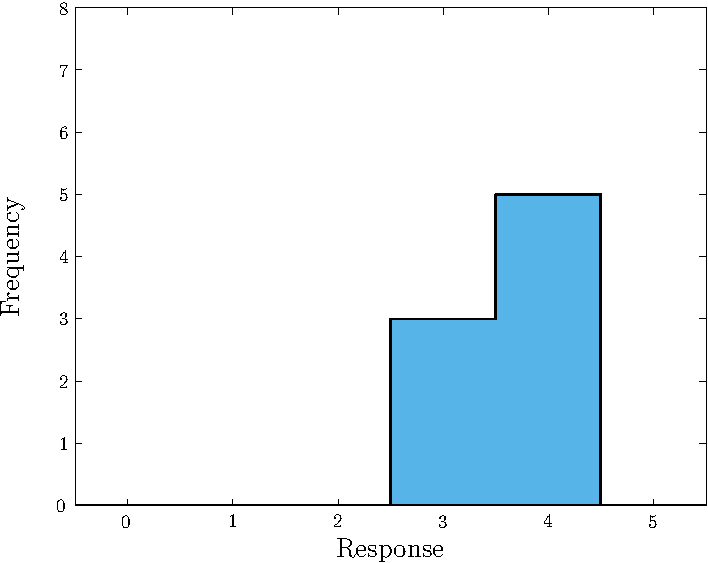
\includegraphics[width=0.47\textwidth]{./figs/Fig_ans_2}} \quad
   \subfigure[{Answers to question 2. Comfort in tutorials ($0$ is uncomfortable, $5$ is comfortable). The mean of the distribution is $4.1$ and the standard deviation is $0.8$.}]{\label{fig:Q2} 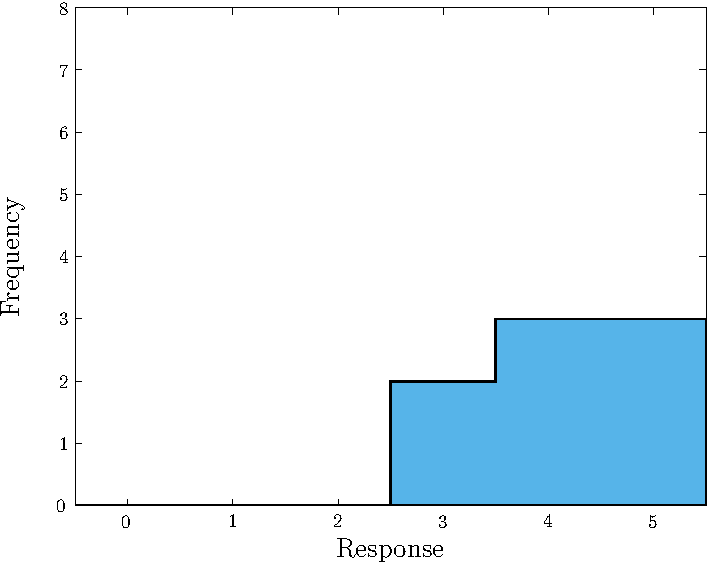
\includegraphics[width=0.47\textwidth]{./figs/Fig_ans_4}} \\ 
   \subfigure[{Answers to question 3. Tutor knowledge ($0$ is low, $5$ is high). The mean of the distribution is $4.9$ and the standard deviation is $0.4$.}]{\label{fig:Q3} 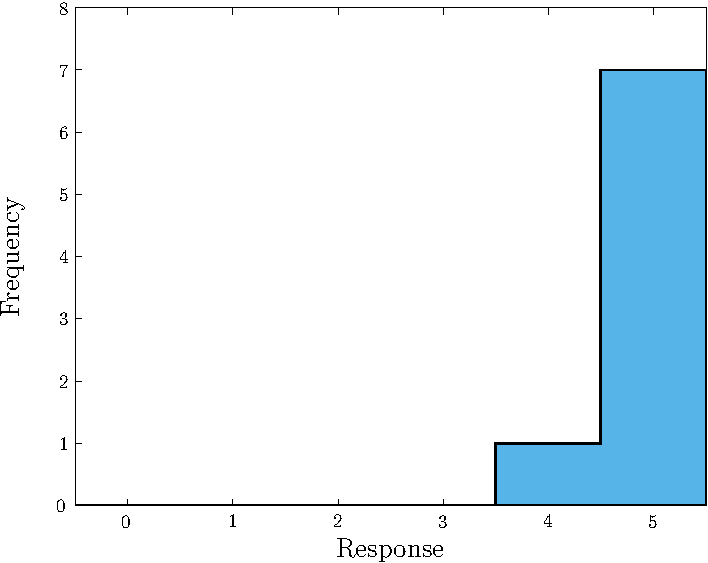
\includegraphics[width=0.47\textwidth]{./figs/Fig_ans_3}} \quad
   \subfigure[{Answers to question 4. Quality of explanation ($0$ is low, $5$ is high). The mean of the distribution is $4.5$ and the standard deviation is $0.5$.}]{\label{fig:Q4} 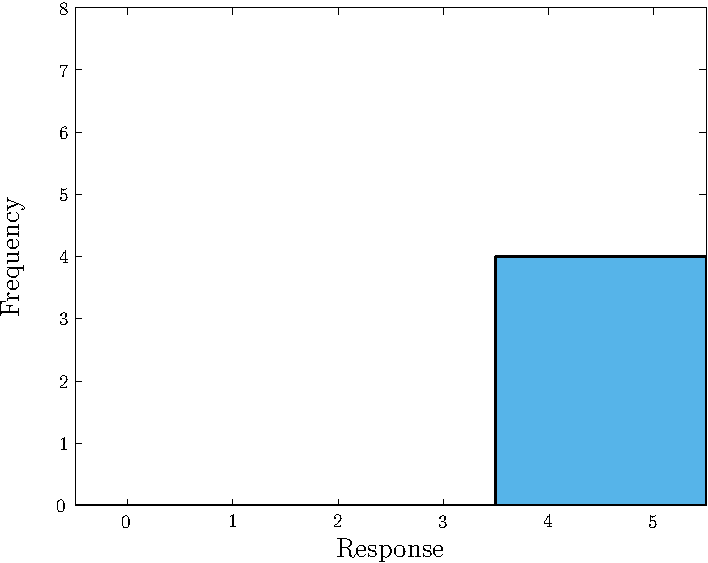
\includegraphics[width=0.47\textwidth]{./figs/Fig_ans_8}} \\ 
   \subfigure[{Answers to question 5. Needs fitting ($0$ is poor, $5$ is well). The mean of the distribution is $4.1$ and the standard deviation is $0.8$.}]{\label{fig:Q5} 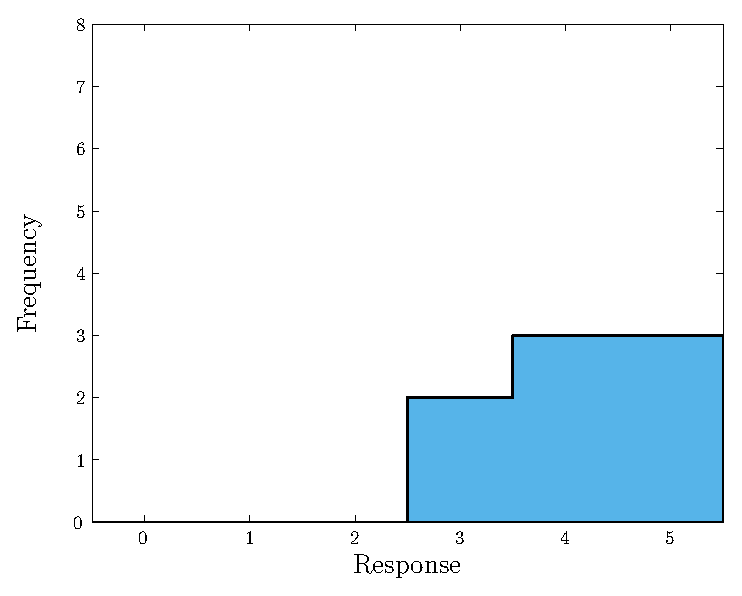
\includegraphics[width=0.47\textwidth]{./figs/Fig_ans_5}} \quad
   \subfigure[{Answers to question 6. Learning from tutorials ($0$ is none, $5$ is lots). The mean of the distribution is $3.6$ and the standard deviation is $1.0$.}]{\label{fig:Q6} 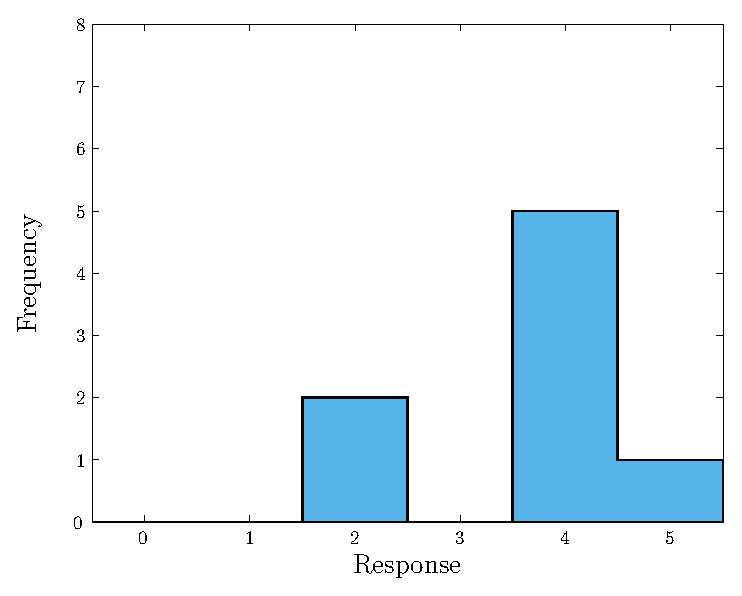
\includegraphics[width=0.47\textwidth]{./figs/Fig_ans_1}} \\
\caption{Student responses to questions 1--6 as described in \tabref{form1}. These questions address tutorials and my teaching of them.}
  \label{fig:plot-A}
\end{figure}

Question 2 (\figref{Q2}) asks how comfortable students are in tutorials. I would hope that most feel happy in tutorials, and that I foster a healthy atmosphere to learn in. None of the students claim to uncomfortable in tutorials, but two do indicate only marginal comfort. There could be multiple explanations for these, perhaps the students are shy and dislike being asked questions or are self-conscious in the group. One of these responses could be from my international student, who could find conversing in a foreign language stressful. Alternatively, it could be that my female students are self-conscious in a male-dominated environment \citep{Gonsalves2014,Gonsalves2014a}. Neither student offers further comment on this point, so I cannot be certain of the reason, it could be something as simple as students not liking a Friday morning time-slot. However, these responses encourage me to be mindful of the diversity of my students and remember that an environment I find comfortable, need not be as hospitable for others.

Questions 5 (\figref{Q5}) and 6 (\figref{Q6}) asks how well tutorials fit student needs and how much students have learnt from them respectively. Responses are generally positive, but there are a couple of less encouraging results. Two students only marginally have their needs satisfied by tutorials. These are also the two students who are also least comfortable in tutorial. One responded with a $4$ to question 6, indicating that they are learning from tutorials; it may be that they are not learning what they really want to. However, they do not give any feedback to illuminate what this could be. If they were the international student, they could need further language support, but this is just conjecture. The other student answers $2$ to question 6, which is concerning. In answer to question 7, they complain that ``too much time spent on problem sheets during tutorial itself'', and in answer to question 22, they ask to ``Look at different ways/more efficient ways to approach a problem (maybe a problem sheet) that may not have been covered in lectures, i.e.\ learn additional techniques''. This suggests that they are one of the more able students and they are not being sufficiently stretched: they do not learn much, because we largely discuss topics that they already understand. In this case, they should suggest further topics for discussion, but they may not be confident enough to do so (they may be conscious as singling themselves out as more able). One other student gave a $2$ for question 6; however, they gave a $5$ for question 6, indicating that they are happy with tutorials. The only comment they offer is in response to question 23, where they state that they want to continue ``going through topics again on the board''. From these response, we may infer that the student is happy with tutorials, but is sufficiently aware that they do not learn during them, this may instead be done while revising afterwards. Overall, it appears that tutorials are generally fulfilling their needs, but this is difficult with a range of different abilities and learning styles within the groups.

Further addressing the topic of the effectiveness of tutorials, there is one other response the question 7: ``I think covering the things we have done in the week is very good and any questions/difficulties we are having in any area is addressed and explained. I enjoy the tutorials overall and find them very helpful.'' This student answered $5$ and $4$ to questions 5 and 6, and $5$ to question 2, indicating that for some students, tutorials are as useful as I intended. In terms of responses to questions 22--24, three students indicated that they wished to continue discussions of topics from the lectures or problem sheets, and another answered ``Addressing anything we are having trouble with in terms of lectures or essay writing etc.'' to question 23, indicating that they are happy bringing forward difficult topics. One student answered ``Nope'' to both questions 22 and 24, indicating they are completely content with the structure as is. The student who I suspect needs to be stretched more suggested that we stop the ``General overview of what we have been doing in lectures, especially since we take a variety of courses between us now. Instead more on core modules like maths.'' This may indicate that they are concerned about wasting time on modules they are studying, perhaps indicating they are motivated by their own exam responses. I believe it is good for them to learn something from other modules, and since the general indication from other students is that they are happy with the current format of discussion, I am happy in continuing in discussing all the lecture courses, although I shall be conscious that we do not spend too long on a course that is only of interest to a few. From the questionnaire responses, there seems to be little need to change the structure or delivery of tutorials.

Discussions in the PRTs lead to similar conclusions. Students commented on how the student-focus of tutorials was good, that they liked tutorials, and that they liked talking about difficult topics. Two commented on how going through problems on the board was useful, but one said that we spent too long on problem sheets. These broadly mirror responses to the questions 22--24.

Answers to question 1 (\figref{Q1}) indicate that tutorials are only viewed as moderately important. This surprised me, as I valued supervisions highly (see \chapref{intro}). Tutorials are where students receive feedback from their problem sheets, and provide a venue for small-group discussions with an academic. Such small-group contact time is scarce, they only have one hour a week compared with the three hours I had during my second year as an undergraduate, hence it seemed counter-intuitive that it was not valued. However, this could reflect a deficiency in the question, since it is difficult to assess importance without a reference point.

Question 33 was designed to correct this by asking students to compare the different aspects of their course. I would expect tutorials to fall somewhere in the middle, I would rank them behind problem sets and private study, approximately on a par with lectures. The ranking of tutorials is shown in \figref{student-tutor-rank} and all responses to are shown in \figref{student-rank}.
\begin{figure}
  \centering
   \subfigure[{Ranking of tutorials by my students. The mean of the distribution is $5.3$ and the standard deviation is $0.8$.}]{\label{fig:student-tutor-rank} 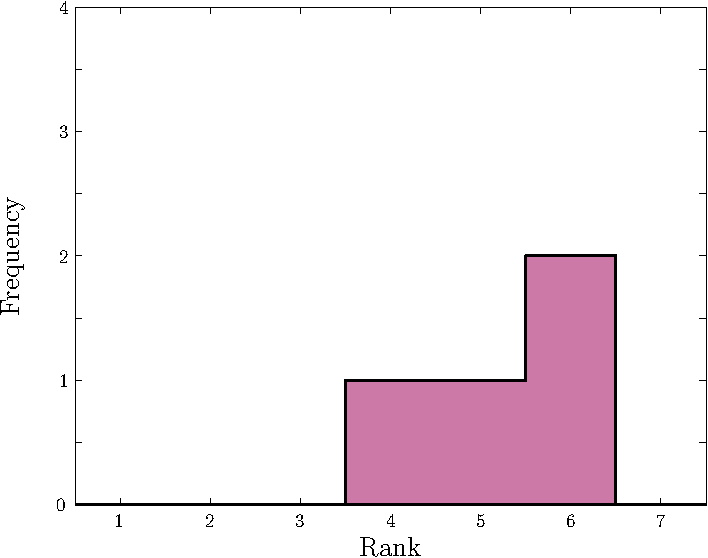
\includegraphics[width=0.47\textwidth]{./figs/Fig_stu_4}} \quad
   \subfigure[{Ranking of tutorials/supervisions by physicists. The mean of the distribution is $4.1$ and the standard deviation is $1.9$.}]{\label{fig:friend-tutor-rank} 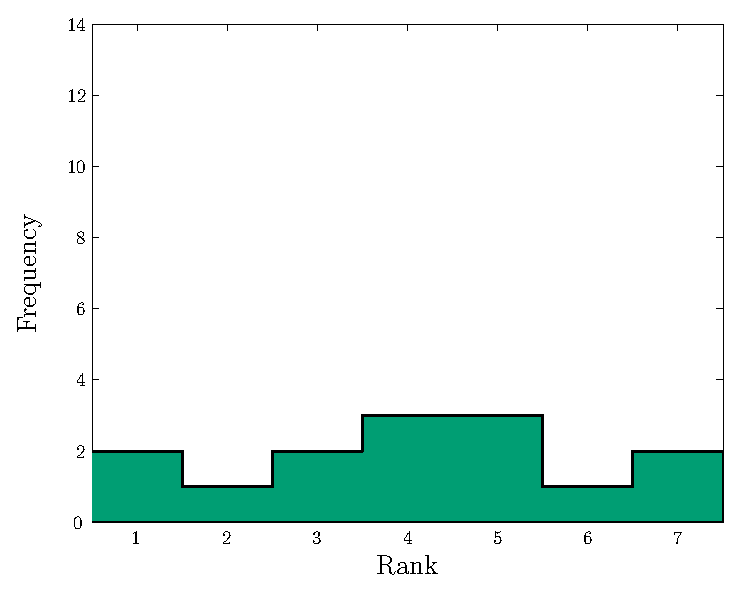
\includegraphics[width=0.47\textwidth]{./figs/Fig_friend_4}}
\caption{Relative ranking of SGT learning in answer to question 33, as described in \tabref{form2}. Rankings for the other components of the course are given in \figref{student-rank} and \figref{friend-rank} as determined by my students and my informal sample of physicists respectively.}
  \label{fig:tutor-rank}
\end{figure}
\begin{figure}
  \centering
   \subfigure[{Ranking of lectures. The mean of the distribution is $4.0$ and the standard deviation is $2.2$.}]{\label{fig:student-lecture-rank} 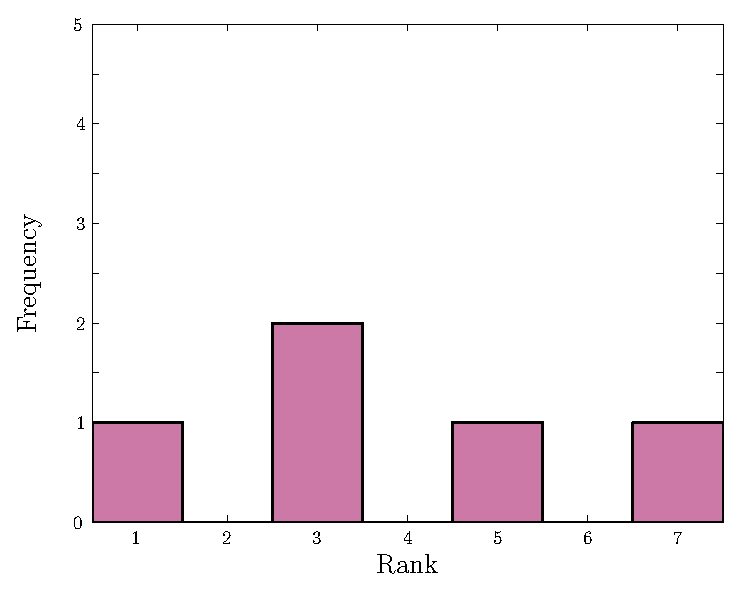
\includegraphics[width=0.47\textwidth]{./figs/Fig_stu_1}} \quad
   \subfigure[{Ranking of labs/practicals. The mean of the distribution is $5.8$ and the standard deviation is $1.1$.}]{\label{fig:student-lab-rank} 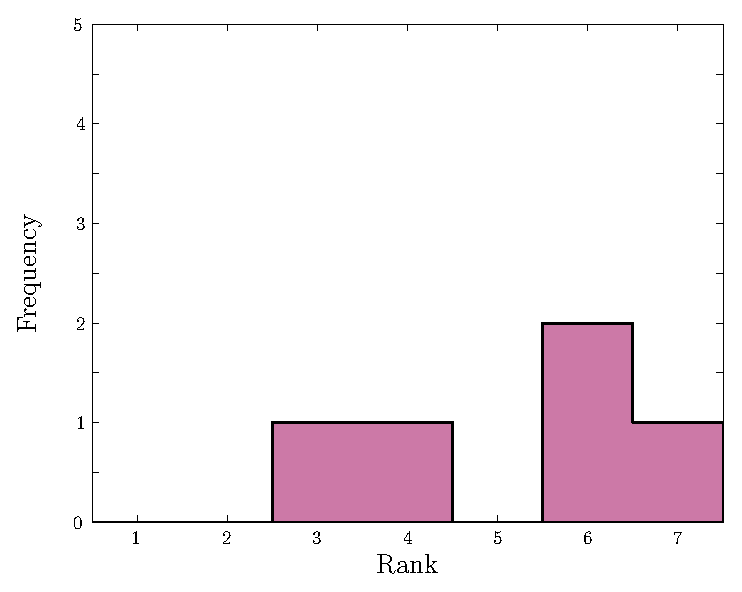
\includegraphics[width=0.47\textwidth]{./figs/Fig_stu_2}} \\ 
   \subfigure[{Ranking of problem sets/assessments. The mean of the distribution is $2.5$ and the standard deviation is $0.9$.}]{\label{fig:student-problem-rank} 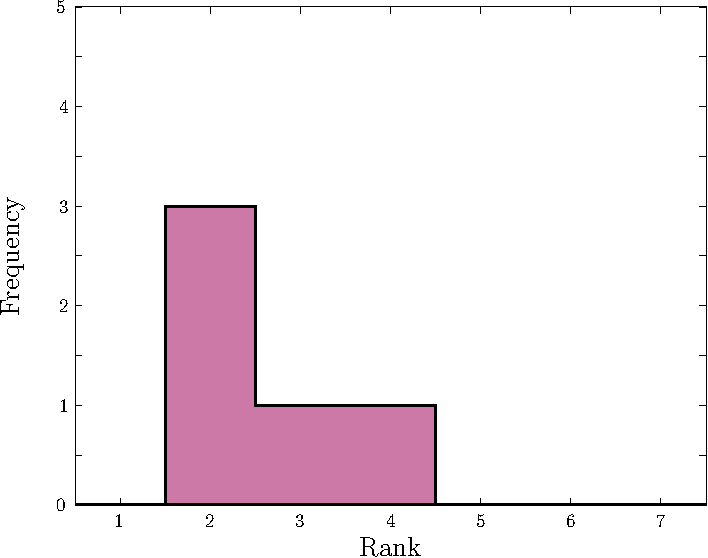
\includegraphics[width=0.47\textwidth]{./figs/Fig_stu_3}} \quad
   \subfigure[{Ranking of private study. The mean of the distribution is $2.0$ and the standard deviation is $1.0$.}]{\label{fig:student-study-rank} 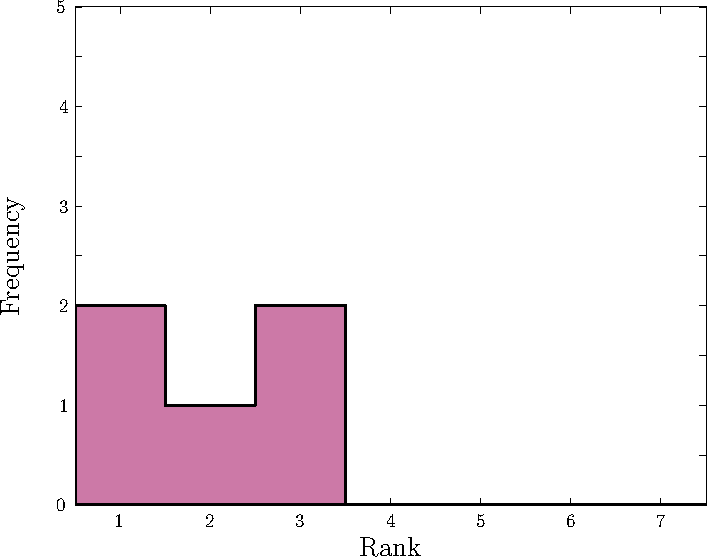
\includegraphics[width=0.47\textwidth]{./figs/Fig_stu_5}} \\ 
   \subfigure[{Ranking of project work. The mean of the distribution is $6.0$ and the standard deviation is $1.0$.}]{\label{fig:student-project-rank} 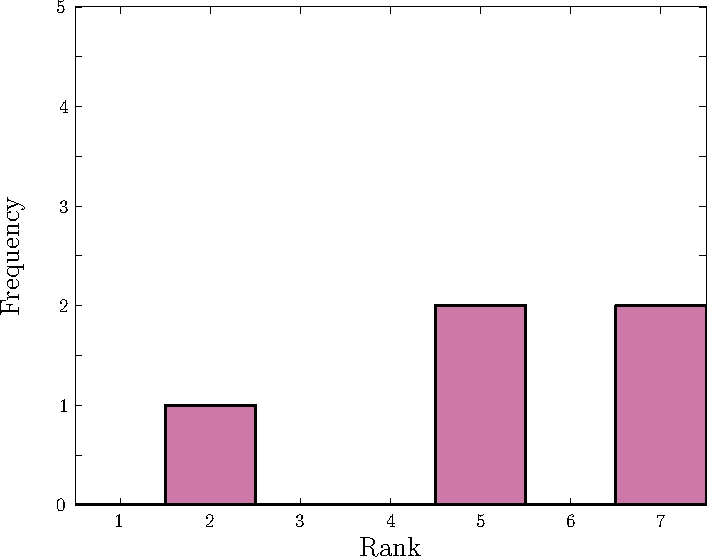
\includegraphics[width=0.47\textwidth]{./figs/Fig_stu_6}} \quad
   \subfigure[{Ranking of exams. The mean of the distribution is $2.5$ and the standard deviation is $1.1$.}]{\label{fig:student-exam-rank} 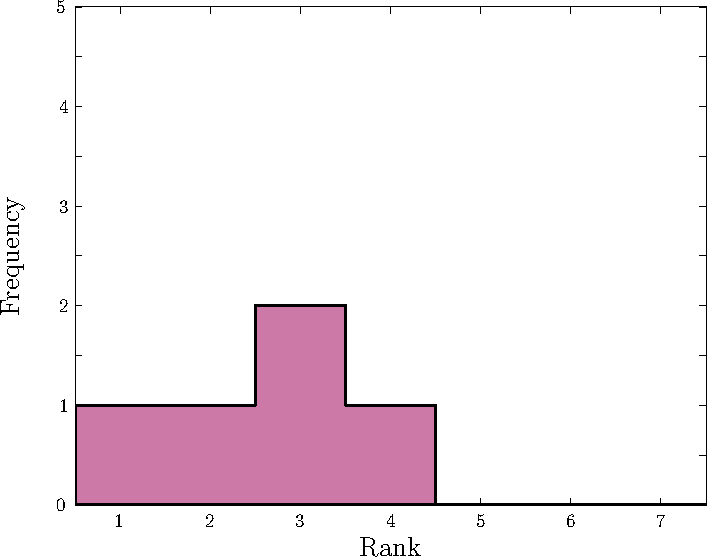
\includegraphics[width=0.47\textwidth]{./figs/Fig_stu_7}} \\
\caption{Student responses to questions 33 as described in \tabref{form2}. This question asks different components of the course to be ranked in terms of educational value. The rankings for tutorials is shown separately in \figref{student-tutor-rank}.}
  \label{fig:student-rank}
\end{figure}
The responses surprised me, in particular exams, which I would consider the least educational activity, are rated as one of the most educational (\figref{student-exam-rank}), with the same mean ranking as problem sets. There may be two possible explanations for this, either students do find exams useful, possibly because they value highly their final grade for evaluated their performance and my expectations are wrong, or students are thinking about the usefulness of completing past papers, an activity I would have included as part of revision.\footnote{The significance of exams should not be overlooked, the second-year students have $15.5~\mathrm{hours}$ of exams compared to $20~\mathrm{hours}$ of tutorials (excluding the revision session).} I would consider the latter more probable, especially since I had been explaining the benefits of practising exam questions at the end of term (see \apref{plan}). As a sanity check, I invited friends of mine who had studied physics at university to complete a questionnaire composed only of questions 33 and 34.\footnote{The only change was to relabel tutorials as tutorials/supervisions.} I received fourteen responses; we shall describe this sample as a group of physicists, although many will be engaged in non-physics careers. The questionnaire was anonymous, so I do not have data on who completed it, it should represent a cross-section of different universities, although I would expect it to be biased towards Cambridge. I would also expect the sample to be biased towards high-achievers, since I met many of my friends during my graduate studies. This sample is not meant to reflect the population, only to check if my own outlook was an outlier. The ranking of tutorials is shown in \figref{friend-tutor-rank} and all responses to are shown in \figref{friend-rank}. The ranking for exams does reflect my expectations, suggesting that I have likely biased my students by discussing pas papers.
\begin{figure}
  \centering
   \subfigure[{Ranking of lectures. The mean of the distribution is $4.3$ and the standard deviation is $1.5$.}]{\label{fig:friend-lecture-rank} 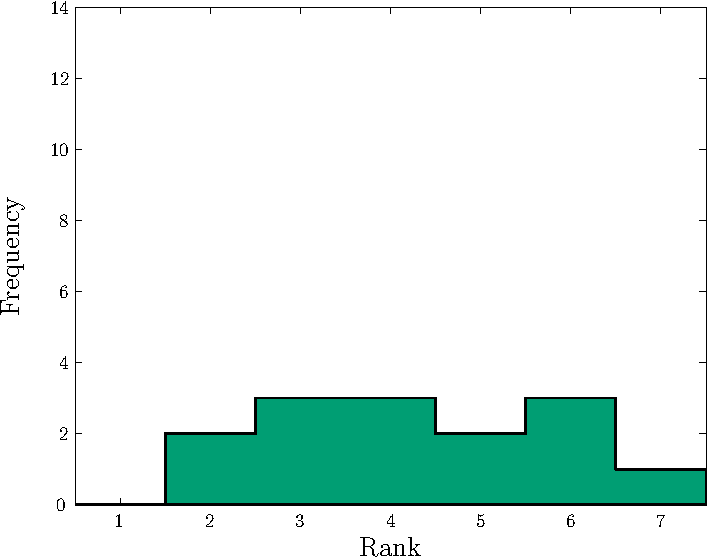
\includegraphics[width=0.47\textwidth]{./figs/Fig_friend_1}} \quad
   \subfigure[{Ranking of labs/practicals. The mean of the distribution is $5.0$ and the standard deviation is $1.6$.}]{\label{fig:friend-lab-rank} 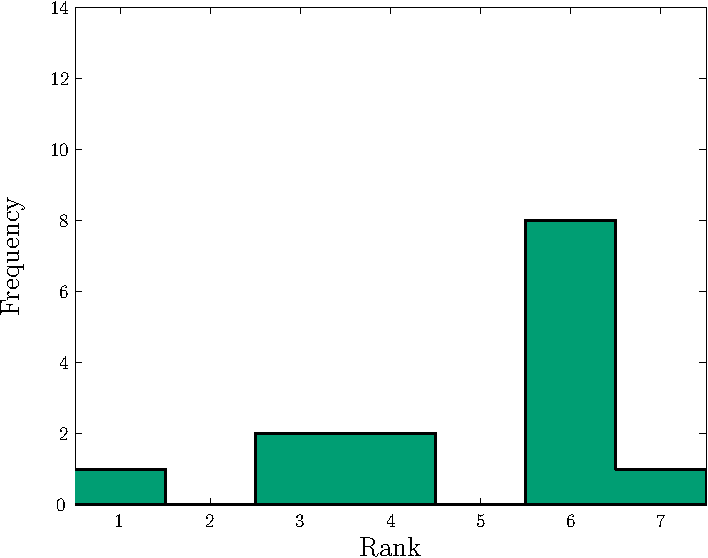
\includegraphics[width=0.47\textwidth]{./figs/Fig_friend_2}} \\ 
   \subfigure[{Ranking of problem sets/assessments. The mean of the distribution is $2.1$ and the standard deviation is $1.0$.}]{\label{fig:friend-problem-rank} 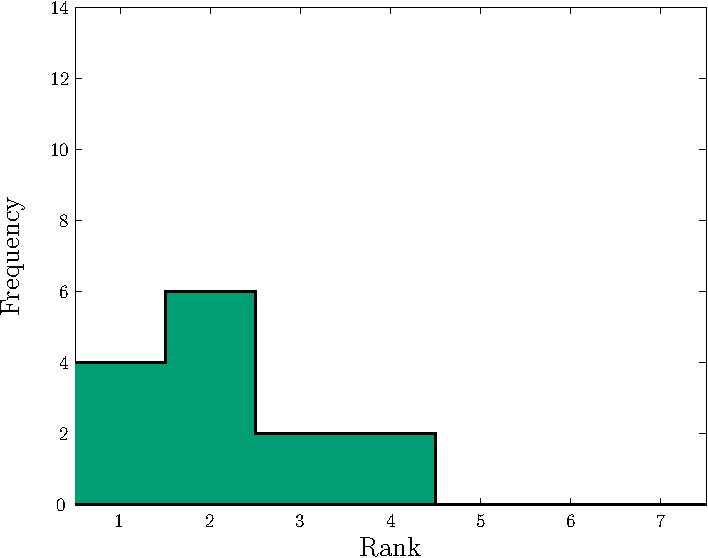
\includegraphics[width=0.47\textwidth]{./figs/Fig_friend_3}} \quad
   \subfigure[{Ranking of private study. The mean of the distribution is $2.8$ and the standard deviation is $1.8$.}]{\label{fig:friend-study-rank} 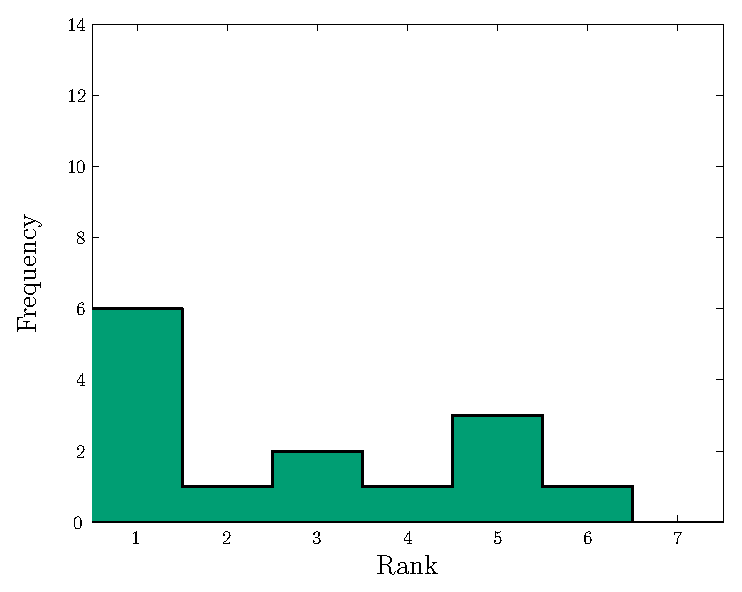
\includegraphics[width=0.47\textwidth]{./figs/Fig_friend_5}} \\ 
   \subfigure[{Ranking of project work. The mean of the distribution is $3.5$ and the standard deviation is $1.7$.}]{\label{fig:friend-project-rank} 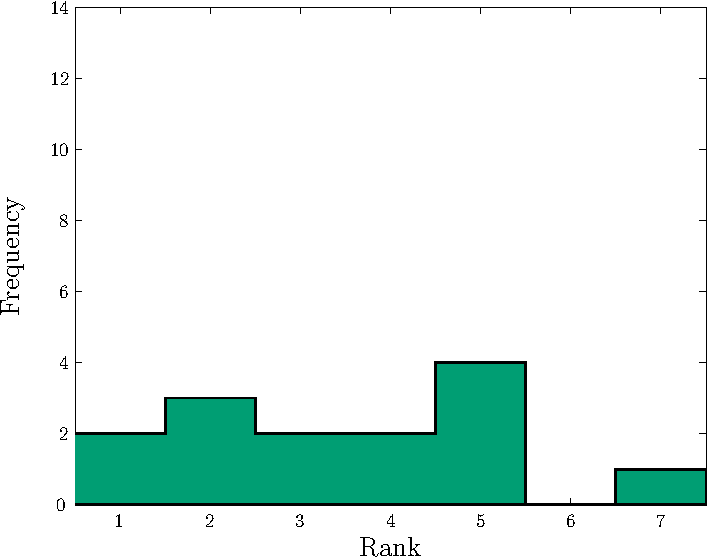
\includegraphics[width=0.47\textwidth]{./figs/Fig_friend_6}} \quad
   \subfigure[{Ranking of exams. The mean of the distribution is $6.9$ and the standard deviation is $0.5$.}]{\label{fig:friend-exam-rank} 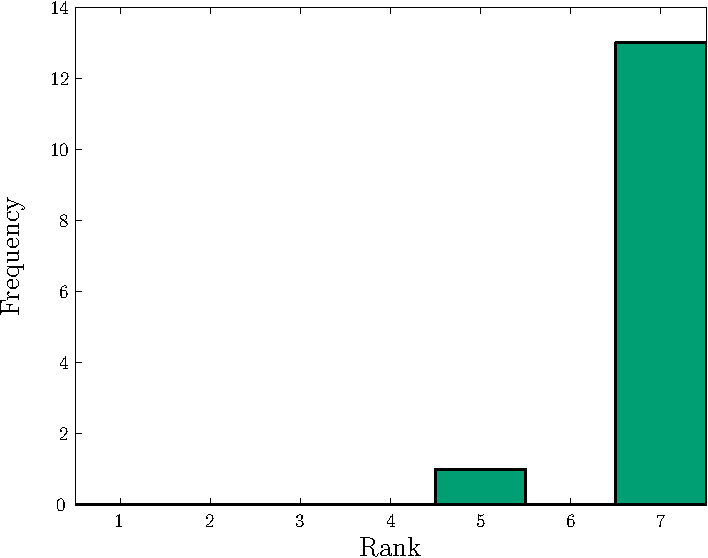
\includegraphics[width=0.47\textwidth]{./figs/Fig_friend_7}} \\
\caption{Responses to questions 33 from an informal sample of physicists. This question asks different components of the course to be ranked in terms of educational value. The rankings for tutorials is shown separately in \figref{friend-tutor-rank}.}
  \label{fig:friend-rank}
\end{figure}

Looking at the results overall, completed problem sets and private study (including completing past papers) are the most useful activities. One of the physicists listed these as most educational, and everything else as least educational. Project work is evaluated differently between the two samples. The students do not consider it educational (\figref{student-project-rank}); the physicists have a mixed experience (\figref{friend-project-rank}), but on average rate it as one of the more educational. The difference is probably explained through the second-year project being limited in scope, and projects in later years having a more significant impact. Excluding exams and projects, labs are the activity where least is learnt (figures \ref{fig:student-lab-rank} and \ref{fig:friend-lab-rank}). Lectures are fairly uniformly distributed between being the most educational and the least educational (figures \ref{fig:student-lecture-rank} and \ref{fig:friend-lectureb-rank}). This may reflect differences in learning styles. Finally, tutorials (\figref{tutor-rank}) have a uniform distribution amongst the physicists, potentially reflecting variation in learning styles and the variation in SGT format, but they are rated low by my students. This is disappointing; however, it should be remembered that most students still learn a considerable amount from tutorials (\figref{Q6}) and that tutorials are only one hour per week. My students do not consider tutorials as useful as I found supervisions, and I must remember this in order to properly calibrate my expectations.

None of my students left a comment in reply to question 34, but I did receive comments from the physicists. One commented that ``Working with others of a similar ability on problems is helpful.'' Cooperative learning has been found to improve student attainment (\citealt{Qin1995}; \citealt[chapter 2]{Falchikov2001}; \citealt{Cabrera2002}), and peer instruction \citep{Roth1994} has been demonstrated to be effective in encouraging learning in physics \citep{Springer1999,Crouch2001,Pilzer2001,Miller2006} and deep learning in general \citep{Marton1976,Wilson2005}; hence this is to be encouraged in students.

Another gave a detailed description of how they learnt through different activities: ``Past papers (or tripos-type questions generally) would come in around problems and lectures, depending on how far through the course you are. Lectures are good when a thing is very new to you, problems help you find what parts you aren't sure of, past papers scare you into getting it right (and are usually fun while you're doing it).'' While I do not agree about past papers being, I agree with the rest. This statement shows why question 33 may be too simplistic, it is not possible to quantify exactly where material is learnt: learning is a process of building up understanding \citep[chapter 2]{Kolb1984}. The foundations of understanding may be laid in lectures, then build upon through completing problem sets with tutorials there to check the stability of the construction, and then the final finishing of the process is during revision at the end of the year. While the different amounts of progress might be made at each stage, each is an important step, without which the others would not work as well.

In closing this section on tutorials, there was one comment in answer to question 25, which solicited any other feedback, that is relevant. A student asked for ``more career focus such as advice on module choices and internship advice'', indicating that employability is a concern for some second-year students.

\subsection{Views on communication skills}\label{sec:comm-results}

Here we examine the student perceptions of communications skills, before proceeding to discuss essay writing in \secref{essay-results}. We will predominantly use responses to questions from section B of the first questionnaire (\tabref{form1}).



Overwork \secref{B-presentation}.

\subsection{Views on essay writing}\label{sec:essay-results}

\section{Conclusion}\label{sec:student-conc}
